\capitulo{4}{Técnicas y herramientas}

En este capítulo se detallan las técnicas y herramientas utilizadas para la \textbf{gestión del flujo} (\autoref{sec:gestionflujo}), el \textbf{soporte de bajo nivel} (\autoref{sec:bajonivel}) sobre las que se ejecutan los servicios, y las herramientas generales (\autoref{sec:herramientasgenerales}).

Como este trabajo es parte de un proyecto mayor, en la \autoref{sec:recogidadatos} se comentan las herramientas para los otros componentes del sistema. En este capítulo se explicarán únicamente las herramientas usadas en este TFM.

\section{Gestión de flujo}\label{sec:gestionflujo}

Uno de los puntos  esenciales de este trabajo es recoger y dirigir los \textit{streams} de vídeo que se reciben. Por tanto, escoger una correcta aplicación para la gestión de este flujo de datos es una parte muy importante dentro de las herramientas.

Dentro de la suite de \textit{Apache} existen varios componentes que se encargan de la gestión del flujos de datos. Se necesitan dos herramientas principales, una capaz de dirigir el flujo y otra para procesarlo.

\subsection{Herramientas para dirigir el flujo}
La primera herramienta necesaria debe ser capaz de dirigir flujos de datos, concretamente flujos de datos serializados para soportar datos más diversos como son las imágenes. También se necesita que sea capaz de desplegar diferentes colas para discriminar fácilmente a los distintos flujos de vídeo entrante.

En la suite de \textit{Apache} existen dos herramientas que gestionan flujos de datos, son: \textit{\textbf{Apache Flume}}~\cite{noauthorapacheflume} y \textit{\textbf{Apache Kafka}}~\cite{noauthorapachenodate}.

\textit{\textbf{Apache Flume}} es una herramienta de gestión de flujo diseñada para hacer una gestión distribuida de manera fiable y altamente disponible de los datos. Proporciona un servicio eficiente para la recogida, agregación y almacenamiento de los datos. Sin embargo, aunque esta herramienta pudiese suplir las necesidades de una gestión de flujo se ha descartado debido a que está optimizada para la gestión de \textit{logs}, concretamente datos codificados como cadenas, y no tiene un sistema de colas.

\textit{\textbf{Apache Kafka}} es un proyecto de intermediación de mensajes que trabaja sobre el patrón publicación-suscripción, funcionando como un sistema de transacciones distribuidas. Incorpora para la implementación de este patrón un sistema de colas para la distribución de mensajes. Aporta una API para el productor, para el consumidor, para el flujo y para el conector. La conexión con \textit{Kafka} se realiza a través del protocolo de la capa de transporte \textit{TCP}. Las diferentes colas que provee \textit{Kafka} se denominan \textit{topics} y son el identificador que utilizan las \textit{APIs} de productor y consumidor para seleccionar la cola sobre la que quieren operar. Para que \textit{Kafka} pueda funcionar necesita estar conectado a un servidor de \textit{Apache Zookeeper}, encargado de la gestión de la memoria y el despliegue de \textit{Kafka}.

Se elije \textit{Apache Kafka} como herramienta para la dirección del flujo al aportar un sistema de colas distribuidas fiable y soportar datos serializados.

\subsection{Herramientas para procesar el flujo}
En segundo lugar se necesita una herramienta capaz de procesar flujos de datos de forma escalable. La suite de \textit{Apache} tiene dos herramientas principales para el procesado de información, son: \textit{\textbf{Apache Hadoop}} y \textit{\textbf{Apache Spark}}, ambas con extensiones para el procesado de flujos.

\textit{\textbf{Apache Spark Streaming}}~\cite{noauthorsparknodate} incluye nativamente una \textit{API} de consumidor de \textit{Kafka} y \textit{Flume}, e integración con los sistemas de ficheros \textit{HDFS} y \textit{S3} entre otras. El funcionamiento interno consiste en crear pequeños lotes de datos para pasarlo al motor de \textit{Spark} y retornar los lotes procesados.

\textit{\textbf{Apache Hadoop Streaming}}~\cite{noauthorhadoop} tiene un funcionamiento similar a \textit{Spark Streaming} pero sin aportar de manera nativa una integración con \textit{Kafka} y \textit{Flume}.

Se ha escogido \textit{Spark Streaming} frente a \textit{Hadoop Streaming} por varios motivos:
\begin{enumerate}
	\item \textit{Spark Streaming} tiene integración con \textit{Kafka} de manera nativa.
	\item \textit{Spark Streaming} hace un uso más intensivo de la memoria RAM, por lo que es mucho más rápido si se cuenta con un equipo con la suficiente memoria disponible para el trabajo deseado.\footnote{El programa final se ha desplegado sobre una máquina con 128 GB de RAM y se ha probado en una de 32 GB de RAM con buenos resultados.}.
\end{enumerate}



\subsection{Servicio de \textit{streaming} de vídeo}

Para comunicar al paciente con el terapeuta asociado y con el sistema de procesado de vídeo se ha utilizado la herramienta \textit{\textbf{Jitsi}}~\cite{tool:jitsi}. Consiste en un servicio de código abierto (Apache 2) para construir y desplegar de manera sencilla una solución de conferencias de vídeo.

Se compone de dos partes: \textit{meet} y \textit{videobridge}. \textit{Jitsi-Meet} es la interfaz web de la aplicación y es usada para que el paciente y el terapeuta se comuniquen. \textit{Jitsi-Videobridge} es la infraestructura de recogida y emisión de vídeo y audio que conectan a ambos clientes.

La razón para usar esta herramienta y no cualquier otro servicio de videoconferencia es porque \textit{Jitsi} es software de código abierto. Gracias a esto podemos desplegar en los servidores locales la herramienta y poder duplicar el vídeo del paciente y que sea dirigido al ingestor de \textit{Kafka}.

\section{Herramientas para el procesado de imágenes}

Para el procesado de las imágenes que componen los vídeos que se van a analizar existe \textit{OpenCV}~\cite{opencv_library}, esta biblioteca de código abierto desarrollada sobre \textit{C++} e integrada en otros muchos lenguajes como \textit{Python}. Debido a la libertad que ofrece al ser \textit{open source}, ser muy versátil, tener una gran trayectoria dentro  y tener una documentación muy completa se ha optado directamente por esta herramienta.

Para la detección de rostros y su correspondiente anonimización, para poder garantizar la privacidad del paciente, se utiliza un modelo de \textit{Caffe}~\cite{jia2014caffe}, concretamente el modelo \textit{res10\_300x300\_ssd\_iter\_140000}. Consiste en una red neuronal convolucional, principal tipo de red neuronal para el análisis de matrices 2D~\cite{lawrence1997face} como son las imágenes.


\subsection{Elección del sistema de compresión de fotogramas}\label{sec:sistemacompresion}

Las principales limitaciones dentro procesamiento de flujos son mantener un uso bajo de memoria dentro de un periodo de tiempo pequeño que garantice poder atender a cada componente del flujo.

Una de las técnicas para garantizar un menor uso de memoria es la compresión de los \textit{bytes} que se ingestan en el sistema de colas aunque esto tiene una mayor carga temporal. Además de la compresión para poder introducir datos en un flujo y luego recuperarlos hace falta serializarlos, es decir, convertirlo en una serie de bytes.

Existen multitud de técnicas de serialización y de compresión de secuencias de \textit{bytes}. Para poder decidir que combinación de estas dos técnicas se van a utilizar se ha buscado que minimicen el tamaño en memoria y utilicen la menor cantidad de tiempo posible.

Para ello se han explorado las siguientes técnicas de serialización:

\begin{itemize}
	\item Serialización nativa: que usa la herramienta \textit{pickle} propia de \textit{Python} para la serialización de objetos.
	\item Codificación \textit{JPG/Exif}~\cite{pennebaker1992jpeg}: estándar de codificación de imágenes que incluye sistema de compresión regulable con pérdidas.
	\item Codificación \textit{PNG}~\cite{boutell1997png}: estándar de codificación de imágenes con sistema de compresión sin pérdidas.
\end{itemize}

Debido a que los estándares \textit{JPG/Exif} y \textit{PNG} son regulables, según el parámetro de compresión interno, se han explorado en el caso de \textit{JPG/Exif} la calidad 95\% y 80\% mientras que con \textit{PNG} las calidades 9 y 5.

Junto con estos sistemas de serialización se han combinado los siguientes algoritmos de compresión:

\begin{itemize}
	\item \textit{LZMA}~\cite{tool:pylzma,seroussi1993lempel}: evolución del algoritmo \textit{LZ77} para la compresión sin pérdida de flujos de datos, evolucionó con la incorporación de las cadenas de Márkov.
	\item \textit{Gzip}~\cite{tool:gzip}: implementación libre del algoritmo de compresión \textit{DEFLATED}, extensión de la versión original de \textit{LZMA} (sin cadenas de Márkov).
	\item \textit{Zlib}~\cite{tool:zlib}: abstracción del algoritmo de compresión \textit{DEFLATED} que usa una menor cantidad de recursos del sistema.
\end{itemize}

Para hacer la prueba se utilizaron dos videos con una duración total entre los dos de 13 minutos, con una frecuencia de 15 fotogramas por segundos, un total de 11700 fotogramas. De cada uno de estas imágenes se calculó el tiempo de compresión, el tiempo de descompresión y el tamaño en memoria que ocupaba tras la compresión. De estos resultados se obtuvo el valor medio. En las figuras~\ref{fig:heatmapmemory} y \ref{fig:resultsComp} se pueden observar tres mapas de calor con los resultados de cada experimento.

\begin{figure}[h]
	\centering
	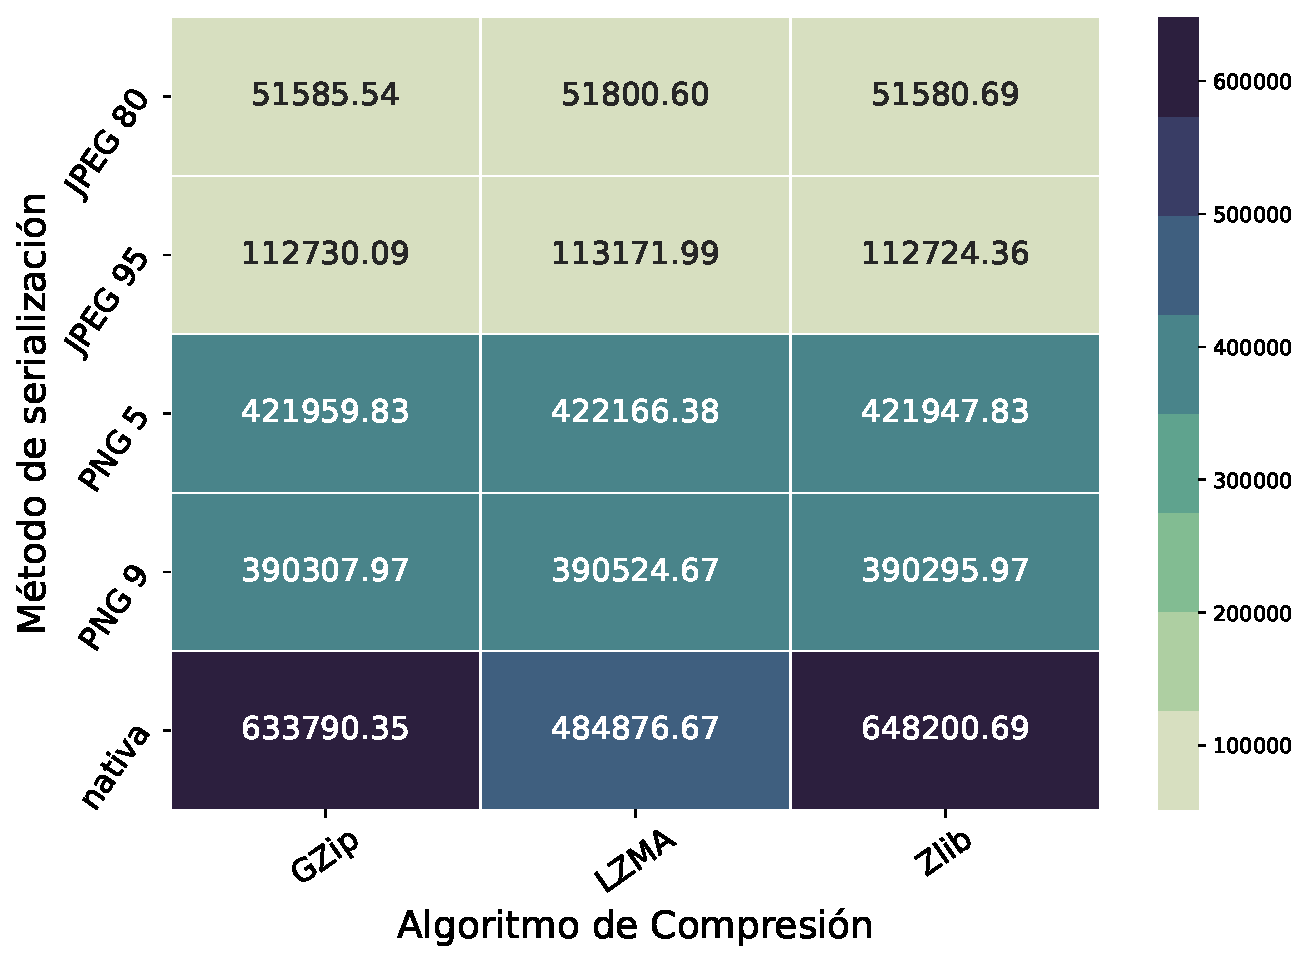
\includegraphics[width=\textwidth]{img/MemoriaMedia.eps}
	\caption{Mapa de calor de la media de espacio consumido (en kilobytes) por fotograma.}
	\label{fig:heatmapmemory}
\end{figure}

\begin{figure}
	\centering
	
	\begin{subfigure}[b]{0.9\textwidth}
		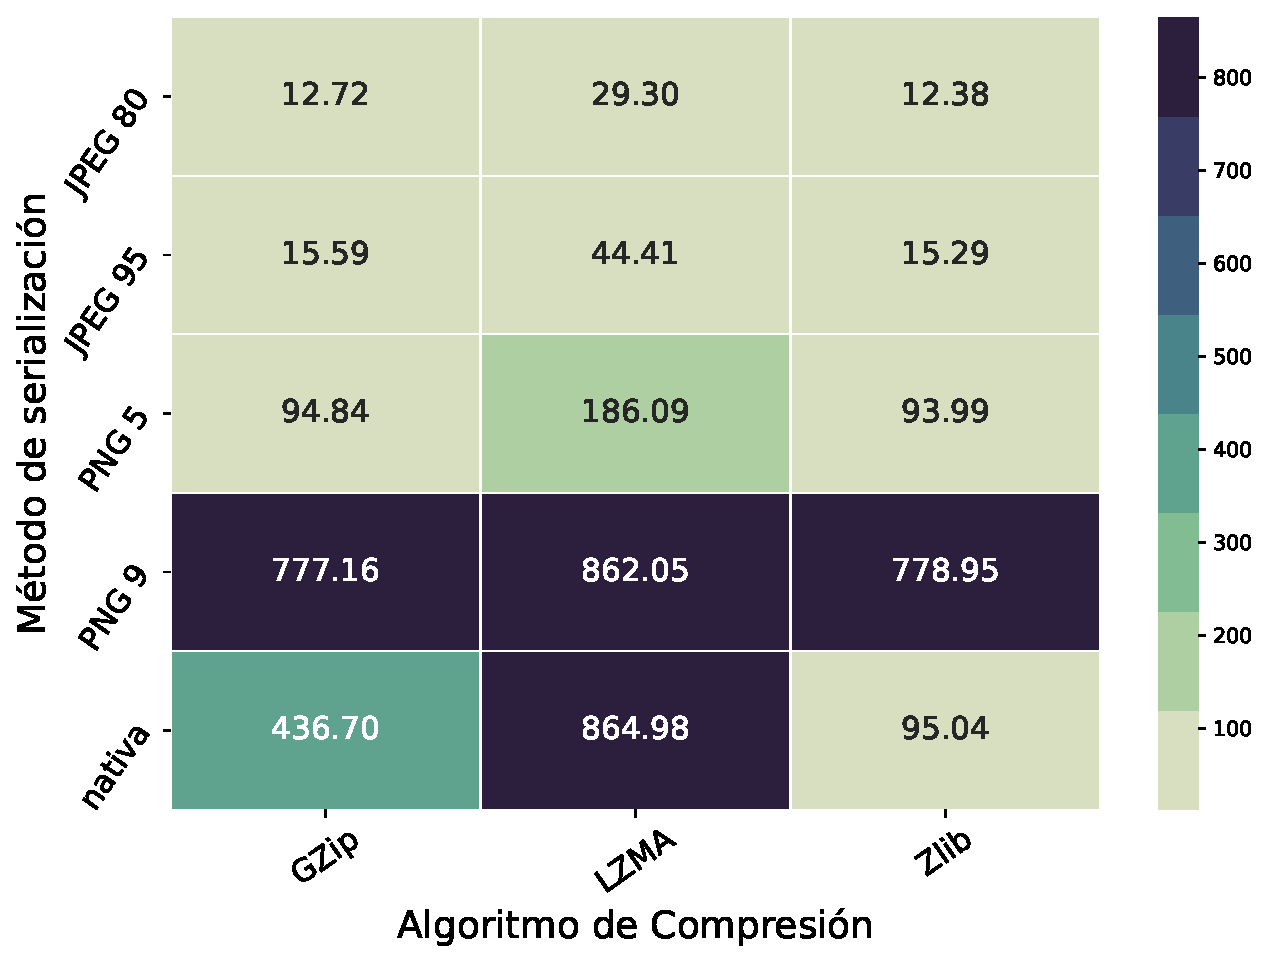
\includegraphics[width=\textwidth]{img/TiempoMedioComp.eps}
		\caption{Media del tiempo necesitado para comprimir fotogramas.}
		\label{fig:heatmaptini}
	\end{subfigure}
	\begin{subfigure}[b]{0.9\textwidth}
		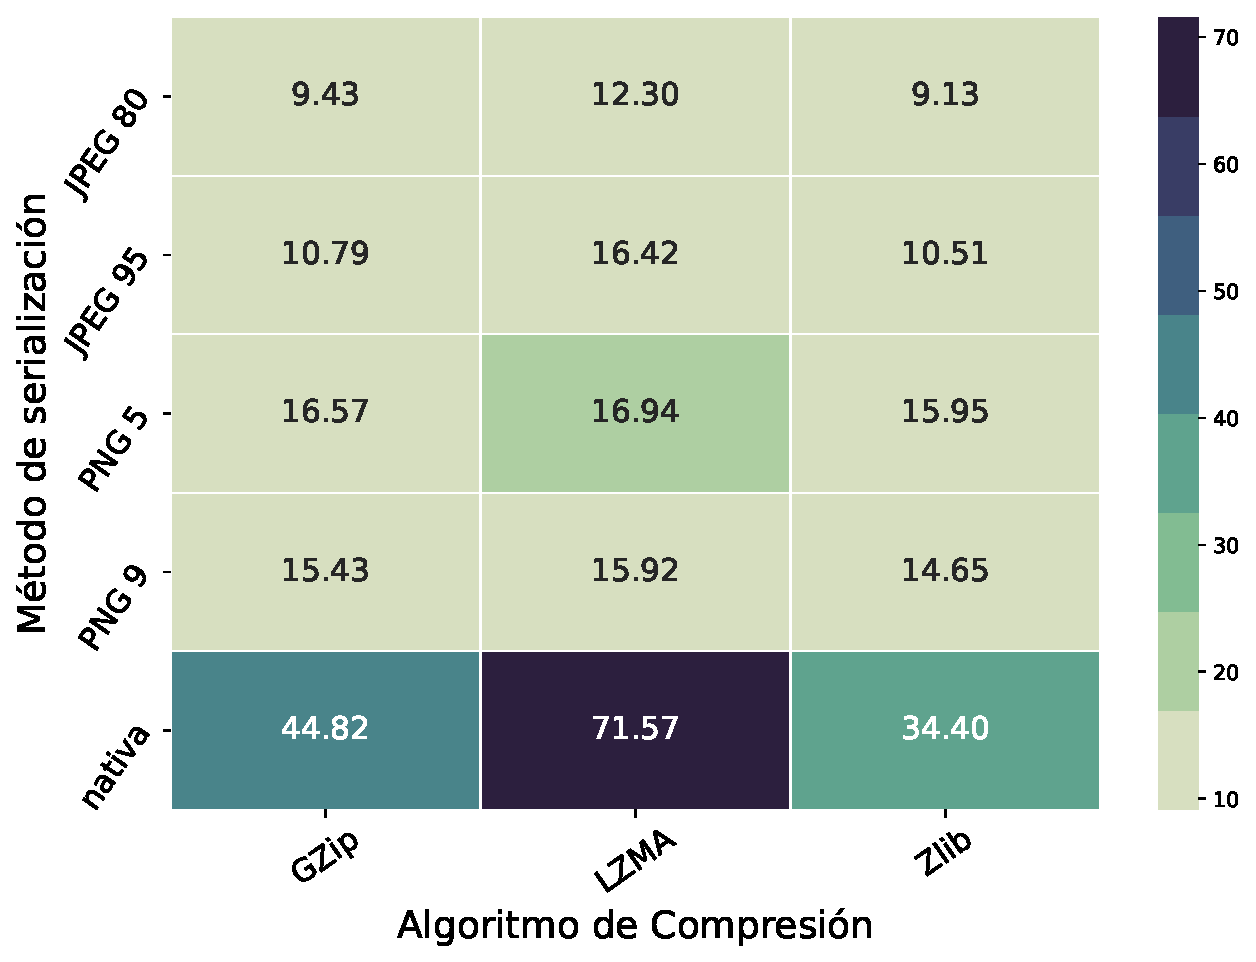
\includegraphics[width=\textwidth]{img/TiempoMedioDes.eps}
		\caption{Media del tiempo necesitado para descomprimir fotogramas.}
		\label{fig:heatmaptfin}
	\end{subfigure}
	\caption{Mapas de calor de los tiempos (en milisegundos) de compresión y descompresión.}
	\label{fig:resultsComp}
\end{figure}

Se puede observar que el algoritmo de compresión \textit{LZMA}, aunque consigue en la mayoría de las veces una muy alta compresión, requiere siempre el mayor tiempo tanto de compresión como de descompresión. De manera similar la serialización nativa mantiene siempre un uso mucho mayor de memoria que el resto de serializaciones, debido principalmente porque tanto \textit{JPG} como \textit{PNG} incorporan un compresor adicional.

Respecto a los algoritmos de compresión \textit{GZip} y \textit{ZLib} las diferencias son muy sutiles tanto en memoria como en tiempo, principalmente por que están basados en el mismo algoritmos.

El uso de \textit{JPG} sobre \textit{PNG} garantiza un uso significativamente menor de memoria aunque a costa de una pérdida de información, sin embargo la pérdida en el caso de \textit{JPEG 95} es despreciable teniendo en cuenta la ventaja que tiene en espacio.

Para este proyecto se utilizarán \textit{JPEG 95} debido a que garantiza una mejor calidad que su contraparte de \textit{JPEG 80} y con una cantidad mucho menor que el resto de serializaciones. Junto a este método se utilizará el algoritmo \textit{ZLib} ya que tiene las mejores métricas temporales.


\section{Infraestructura de bajo nivel}\label{sec:bajonivel}

Otro apartado importante en el despliegue de la aplicación son las herramientas y técnicas a ser usadas para la producción. Para esto se utilizan:

\begin{itemize}
	\item \textit{\textbf{GNU/Linux}}, el sistema operativo más extendido en el entorno de los servidores~\cite{noauthorred2018, zhang2000linux} además de estar disponible en los servidores prestados para la realización de este proyecto\footnote{Se utilizan el servidor \textit{Alpha} del GIR \href{https://admirable-ubu.es/}{ADMIRABLE} para el despliegue de la herramienta de recolección de datos (Procesador \textit{Intel Core i7}-8700, 6 núcleos, 3.2GHz. 64GB de memoria RAM. 2 GPUs GTX 1080Ti y 500GB de disco duro sólido y 6 TB de disco duro magnético) y el servidor \textit{Gamma} del mismo grupo para el despliegue de las colas y el procesado de la información (Procesador Intel Xeon, 10 núcleos. 128 GB de memoria RAM. 3 GPU Nvidia Titan Xp)}.
	\item \textit{\textbf{Docker}}, un software de gestión de contenedores estandarizados, semejante a los entornos \textit{chroot} que facilita la virtualización de software en un entorno seguro y ligero. Sobre este motor se ejecutarán las aplicaciones del entorno de \textit{Apache Spark}~\cite{juez2019docker}, \textit{Apache Kafka}~\cite{confluentic2020docker} además de la aplicación desarrollada para el cumplimiento de los objetivos.
	\item \textit{\textbf{Ngrok}}, software que ofrece un tunel TCP y HTTP sobre un servicio que no tiene acceso al exterior. Es usado para poder acceder al servicio web desde fuera de la universidad.
\end{itemize}

\section{Herramientas generales}\label{sec:herramientasgenerales}

Para el desarrollo general del proyecto se han utilizado las siguientes herramientas:

\begin{itemize}
	\item \textbf{Visual Studio Code}: Editor de código genérico de código abierto (MIT).
	\item \textbf{Overleaf}: Editor de \LaTeX{} online para el trabajo colaborativo.
	\item \textbf{\TeX{}Studio}: Editor de \LaTeX{} de código abierto (GPLv2).
    \item \textbf{Dia}: Editor de diagramas genérico de código abierto (GPL).
    \item \textbf{Filezilla}: Aplicación para la trasferencia de ficheros sobre \textit{FTP} y \textit{SFTP} de código abierto (GPLv2).
    \item \textbf{GitHub}: Servicio online de \textit{hosting} para repositorios Git.
\end{itemize}
